% Section: Using Abisko
% Latex file for the MPI Course at HPC2N Umea 
%    Elaborated by P. Ojeda
%

%########################  NEW SECTION  ########################
\section{Using Abisko}

%%%%%%%%%%%%%%%%% NEW  SLIDE
\begin{frame}
	\frametitle{Abisko}
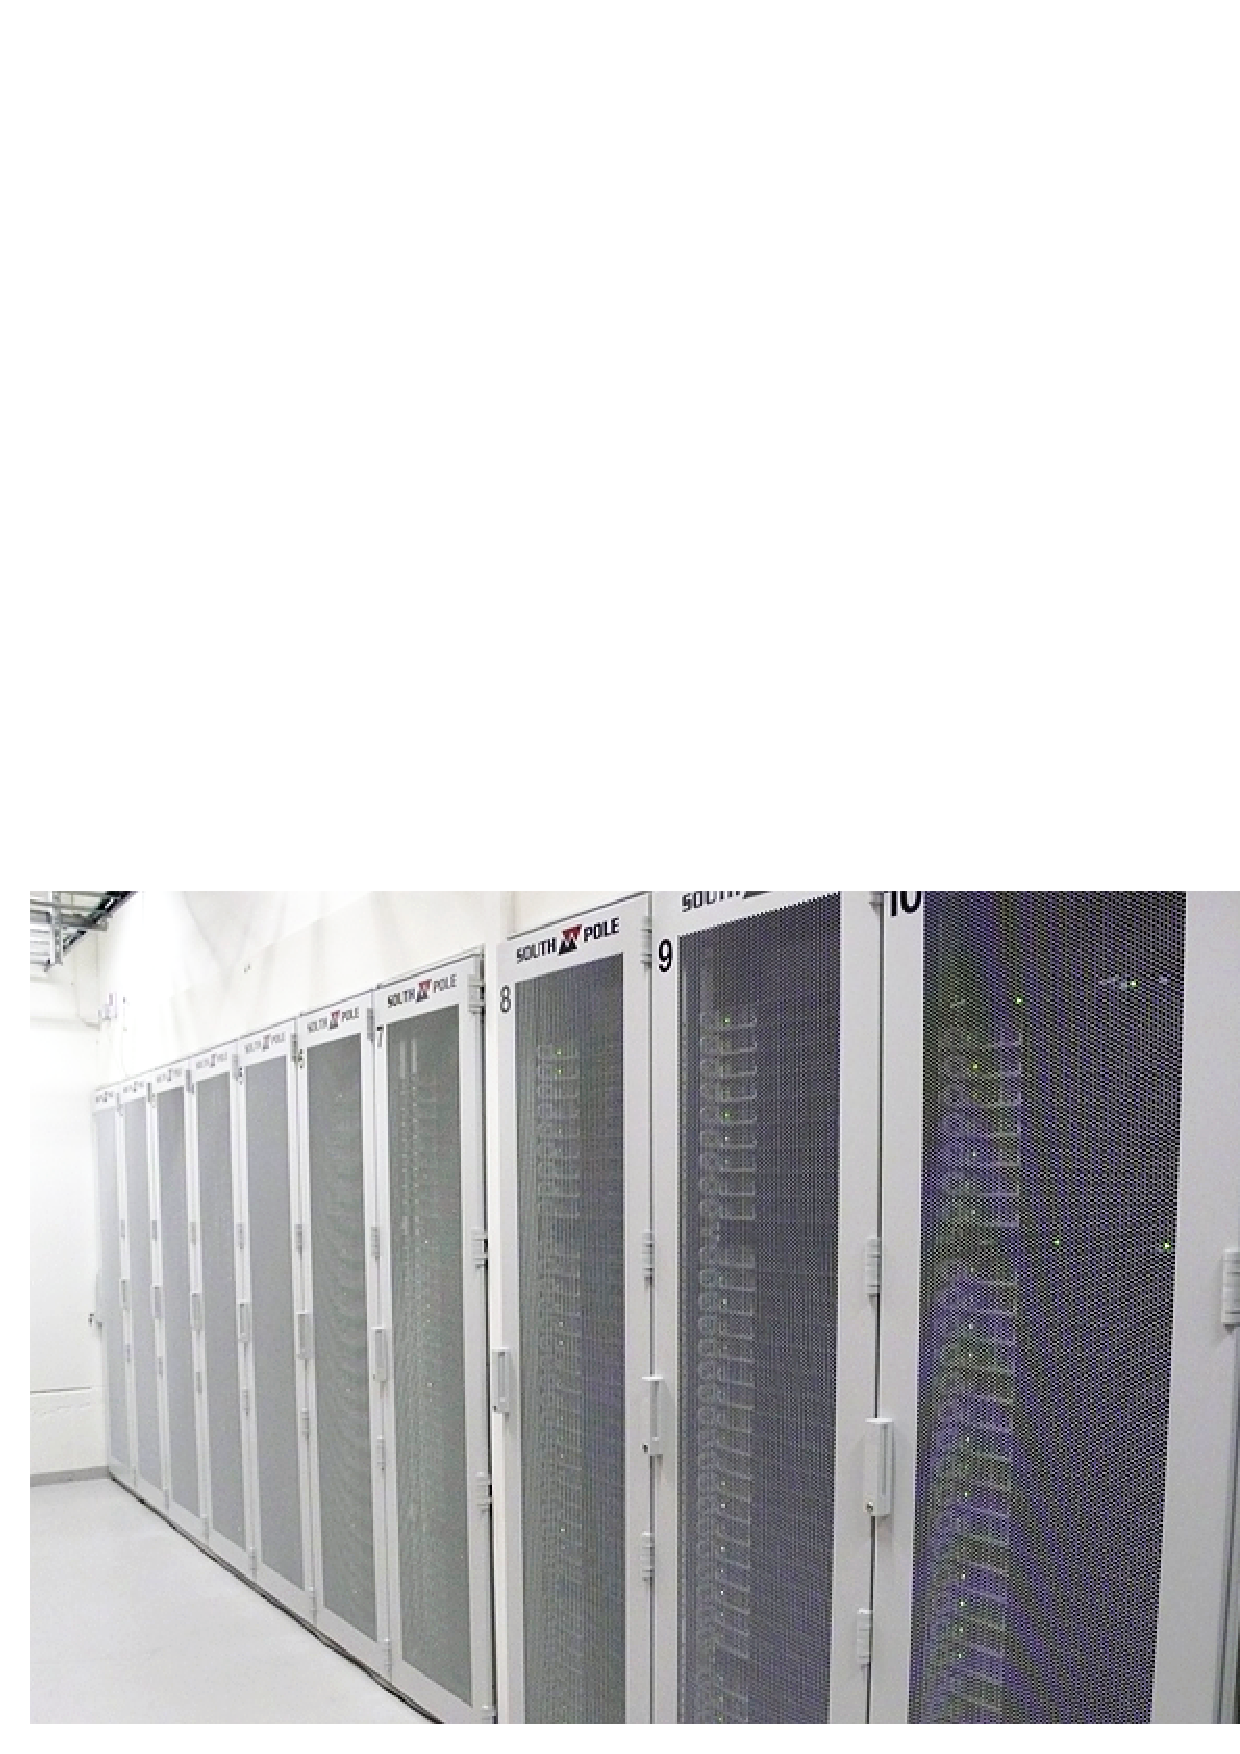
\includegraphics[width=4.5cm]{images/abisko.jpg}
	\begin{itemize}
		\item	332 nodes/15936 cores
		\item	10 fat nodes (512 GB RAM), 318 thin nodes (128 GB RAM)
		\item	CPUs: (thin) 4 x AMD Opteron 6238 (Interlagos) 12 core (2.6 GHz)
		\item	CPUs: (fat) 4 x AMD Opteron 6344 (Abu Dhabi) 12 core (2.6 GHz)
		\item	Interconnect: Infiniband QDR, 40Gb/s, Mellanox
		\item	Installed 2011
	\end{itemize}
\end{frame}

%%%%%%%%%%%%%%%%% NEW  SLIDE
\begin{frame}
	\frametitle{Abisko}
	\begin{itemize}
		\item	Application software: Abinit, Ansys, DDT, Espresso,
				Gamess, Gaussian, Gromacs, HDF5, Matlab, NetCDF,
				NWChem, Octave, PETSc, R, Siesta, VASP, WRF, ...
		\item	Num. and Comm. libraries: BLACS, FFTW, BLAS, LAPACK,
				ScaLAPACK, ACML, Intel MKL, ParMETIS, RECSY, SLICOT, ...
		\item	MPI: OpenMPI, Intel MPI
		\item	Other software on request
	\end{itemize}
\end{frame}


%%%%%%%%%%%%%%%%% NEW  SLIDE
\begin{frame}
	\frametitle{Kebnekaise}
\begin{columns}
	\column[T]{5cm}

\includegraphics[width=5cm]{images/kebnekaise.eps}
	\begin{itemize}
		\item	13 racks, Mixed system:
		\item	432 Intel Broadwell, E5-2690v4 (2x14 cores/node), 128 GB/node
		\item	36 Intel Broadwell + NVidia K80 GPUs (32 with 2/node, 4 with 4/node)
	\end{itemize}
	\column[T]{5cm}
	\begin{itemize}
		\item	20 Intel Haswell E7-4850v3, (4x14 cores/node), 3 TB/node (fat nodes)
		\item	36 Intel KNL: 7250 SKU (68 cores, 1.4/1.2 Ghz/AVX), 192 GB/node
		\item	Interconnect: Mellanox Infiniband FDR
	        \item   OS: Linux Ubuntu
	        \item   Installation: Summer/Fall 2016
	\end{itemize}
\end{columns}
\end{frame}



%------------------  NEW SUBSECTION ------------------
\subsection{Connecting}

%%%%%%%%%%%%%%%%% NEW  SLIDE
\begin{frame}
	\frametitle{Connecting from a Windows System}

	You need an ssh client to connect.
	\begin{itemize}
		\item	PuTTY
		\item	Cygwin
	\end{itemize}

	If you want to open graphical displays, you need an X11 server
	\begin{itemize}
		\item	Xming
		\item	Cygwin
	\end{itemize}

	Transferring files (sftp or scp)
	\begin{itemize}
		\item	WinSCP
		\item	FileZilla (only sftp)
		\item	PSCP/PSFTP
	\end{itemize}

\end{frame}

%%%%%%%%%%%%%%%%% NEW  SLIDE
\begin{frame}
	\frametitle{Connecting from a UNIX/Linux System}

	\begin{itemize}
		\item	Login with ssh:\\
		 \texttt{local> ssh username@abisko.hpc2n.umu.se}
		\item	If you want to open graphical displays, you need
				to enable X11 Forwarding:\\
		 \texttt{local> ssh -X username@abisko.hpc2n.umu.se}
		\item	Use scp for file transfer:\\
		 \texttt{local> scp username@abisko.hpc2n.umu.se:file /tmp}\\
		 \texttt{local> scp file username@abisko.hpc2n.umu.se:file}
	\end{itemize}

\end{frame}

%------------------  NEW SUBSECTION ------------------
\subsection{Modules}

%%%%%%%%%%%%%%%%% NEW  SLIDE
\begin{frame}
	\frametitle{Modules}

	\begin{itemize}
		\item	Many versions of software packages
		\item	Use a tool called modules
			\begin{itemize}
				\item	Can choose a combination of libraries and compilers
						that will work together
				\item	Changes the environment
				\item	User guide and man-page
			\end{itemize}
	\end{itemize}

\end{frame}
%%%%%%%%%%%%%%%%% NEW  SLIDE
\begin{frame}
	\frametitle{Modules}

	\begin{itemize}
		\item	Some useful module commands
			\begin{description}
				\item[help]		list all module commands
				\item[show]		display information on a module
				\item[add]		add a module to the environment
				\item[rm]		remove a module from the environment
				\item[list]		list currently activated modules
				\item[avail]	list all modules that exist on the system
			\end{description}
		\item	Examples
			\begin{itemize}
				\item	\texttt{module add pgi}\\
						will add the latest version of the Portland compilers
				\item	\texttt{module add openmpi/pgi}\\
						will add the latest version of openmpi
						(suitable for the current machine)
						that was built with the Portland compilers
			\end{itemize}
	\end{itemize}

\end{frame}

%------------------  NEW SUBSECTION ------------------
\subsection{File Systems}

%%%%%%%%%%%%%%%%% NEW  SLIDE
\begin{frame}
	\frametitle{File Systems}


\begin{columns}
	\column[T]{5cm}
		There are 2 file systems\\
		AFS
		\begin{itemize}
			\item	Your home directory
			\item	Backed up regularly
			\item	NOT accessable by the batch system
		\end{itemize}
		PFS
		\begin{itemize}
			\item	Parallel file system
			\item	NO BACKUP
			\item	Accessable by the batch system
		\end{itemize}
	\column[T]{5cm}
		\vspace*{-1cm}
		\includegraphics[width=6.5cm]{images/filesystem.eps}
\end{columns}
\end{frame}

\begin{frame}
    \frametitle{PFS}

	\begin{itemize}
		\item	Offers high performance when accessed from the nodes
		\item	To create soft link from your home directory to your
				corresponding home on the parallel file system\\
				\texttt{ln~-s~/pfs/nobackup\$HOME~\$HOME/pfs}
		\item	Then if you use\\
				\texttt{cd pfs}\\
				from your home directory
				you will end up in your "parallel" home directory
				
	\end{itemize}
	
\end{frame}


%------------------  NEW SUBSECTION ------------------
\subsection{Batch System}

%%%%%%%%%%%%%%%%% NEW  SLIDE
\begin{frame}
	\frametitle{Batch System (SLURM)}

	\begin{itemize}
		\item	Large/parallel programs, run through the batch system
		\item	Keeps track of available system resources
		\item	Takes care of scheduling jobs of multiple users,
				running tasks simultaneously
		\item	Enforces local system resource usage and job scheduling policies
		\item	Users submit to a queue (running, idle, blocked)
	\end{itemize}

\end{frame}

\begin{frame}[fragile]
	\frametitle{Job script}
  
\begin{columns}
	\column[T]{5cm}
	\only<1->{\texttt{\#!/bin/bash}\\}
	\only<1,3->{\texttt{\#SBATCH~-A~SNICYYYY-XX-NN}\\}
	\only<2>{\hilite{\texttt{\#SBATCH~-A~SNICYYYY-XX-NN}}\\}

	\only<1-2,5-7,9->{\texttt{\#SBATCH -n 48}\\}
	\only<3-4,8>{\hilite{\texttt{\#SBATCH -n 48}}\\}

	\only<1-4,6->{\texttt{\#SBATCH --time=01:00:00}\\}
	\only<5>{\hilite{\texttt{\#SBATCH --time=01:00:00}}\\}

	\only<1->{\texttt{ }\\}

	\only<1-5,7,9->{\texttt{module add openmpi/psc}\\}
	\only<6,8>{\hilite{\texttt{module add openmpi/psc}}\\}

	\only<1-6,9->{\texttt{srun~./parallel\_prog args}\\}
	\only<7-8>{\hilite{\texttt{srun ./parallel\_prog args}}\\}

	\column[T]{5cm}
	\only<1>{
		\begin{itemize}
			\item	Submitting:\\
					\texttt{sbatch <{\em jobscript}>}
			\item	Show the job queue:\\
					\texttt{squeue [-u {\em username}]}
			\item	Delete a job:\\
					\texttt{scancel <{\em jobid}>}
		\end{itemize}
	}
	\only<2>{
	Your account (-A)
		\begin{itemize}
			\item	The account is your project id
			\item	Low priority if not set
			\item	You can find your project id by running:\\
						\texttt{projinfo}
		\end{itemize}
	}
	\only<3>{
		Number of tasks (-n)
		\begin{itemize}
			\item	The number of tasks is for the most cases
					the number of processes you want to start.
			\item	The default value is one
			\item	e.g. number of MPI tasks
			\item	e.g. number of serial programs
		\end{itemize}
	}
	\only<4>{
		Number of cores per task (-c)
		\begin{itemize}
			\item	For multi threaded applications (OpenMP/pthreads/...)
			\item	indicates the number of cores each task can use
			\item	The default value is one
			\item	Maximum is 48
		\end{itemize}
	}
	\only<5>{
		The run/wallclock time \texttt{D-HH:MM:SS}
		\begin{itemize}
			\item	Runtime (wall clock time) of your job
			\item	Try to estimate correctly
					\begin{itemize}
						\item	Hard limit
						\item	Shorter jobs are more likely to fit into slots
								of unused space faster.
					\end{itemize}
		\end{itemize}
	}
	\only<6>{
		Load modules needed or other things. (This is for your program that is
		compiled with the PathScale compiler and the OpenMPI library.)
	}
	\only<7>{
		Run your MPI application using \texttt{srun}
		\begin{itemize}
			\item	Starts the required number of processes
			\item	Note! If your program is serial it will start many instances
		\end{itemize}
	}
	\only<8>{
		Run your multi threaded application on 36 cores.
		Change the marked lines with:\\
		{\texttt{ }\\}
		{\texttt{\#SBATCH -c 36}\\}
		{\texttt{ }\\}
		{\texttt{export OMP\_NUM\_THREADS=36}\\}
		{\texttt{ }\\}
		{\texttt{./my\_OpenMP\_program args}\\}
	}
	\only<9>{
		Output
		\begin{itemize}
			\item	Put stdout into the file
					\texttt{<{\em jobid}>.out}\\
					\texttt{\#SBATCH~--output=\%J.out}
			\item	Put stderr into the file
					\texttt{<{\em jobid}>.err}\\
					\texttt{\#SBATCH~--error=\%J.err}
			\item	By default both to \texttt{slurm-<{\em jobid}>.out}
		\end{itemize}
		Input
		\begin{itemize}
			\item	Use \texttt{file.txt} as stdin\\
					\texttt{\#SBATCH~--input=file.txt}
		\end{itemize}
	}
\end{columns}

\end{frame}

